\openingarticle
\def\ppages{\pagerange{Forssman:firstpage}{Forssman:lastpage}}
\def\shorttitle{Late Holocine Rockshelter, Botswana}
\def\maintitle{The Late Holocene Occupation of Mafunyane Shelter, Eastern Botswana}
\def\shortauthor{Tim Forssman}
\def\authormail{GETEMAILADRESS@email.com}
\def\affiliation{University of Oxford}
\def\thanknote{\footnote{Rock Art Research Institute, School of Geography, Archaeology and Environmental Studies, University of the Witwatersrand, Johannesburg, 2050 South Africa 
DPhil Research carried out at the University of Oxford (UK)}}
%--------------------------------------------------------------
\mychapter{\maintitle}
\begin{center}
	{\Large\scshape\shortauthor \thanknote}\\[1em]
	\email \\
	\affiliation
\end{center}
\vspace{3em}
\midarticle
%--------------------------------------------------------------
\label{Forssman:firstpage}

%----------------------------------------------------------------------------------------
	%----------------------------------------------------------------------------------------
	%	ABSTRACT
	%----------------------------------------------------------------------------------------
\begin{myabstract}
		\noindent  Mafunyane Shelter is a small rockshelter situated in eastern Botswana along the Limpopo River. The site was occupied from possibly the first centuries \AD until the Leopard’s Kopje period, \AD 1000 to 1300. 
		Excavations revealed an extensive Later Stone Age (LSA) assemblage including stone tools, beads and a diverse faunal record as well as ceramics, a figurine fragment and various metal and metal-working associated finds. Inside the rockshelter is a limited number of rock markings including paintings, cupules and grooves. The site was originally excavated by \parencite{Walker_1994} but until now has not been dated. Here, new findings from a subsequent excavation are presented along with a revised chronological sequence. 
		The occupation of Mafunyane is discussed and the implications relating to the farmer-associated items such as the ceramics and metal assemblage are considered. The results suggest that an expansion of our research approach might reveal aspects of the LSA seldom occurring at large rockshelter sites, such as specific site utilisation patterns, specialist or craft activities, and the variable social responses from forager-farmer interactions.
		
\keywords[Keywords]{Later Stone Age, stone tools, hunter-gatherers, forager-farmer interactions, Greater Mapungubwe Landscape, eastern Botswana}
	\end{myabstract}

	
	%\section{Introduction}
	\lettrine[nindent=0em,lines=3]{T}{he} Later Stone Age (LSA) sequence of the Greater Mapungubwe Landscape, which includes parts of eastern Botswana, northern South Africa and south-western Zimbabwe (Fig. \ref{fig:Forssmann-Figure01}), has been at the centre of a number of studies \parencites[e.g.][]{Hall_2000}{van Doornum_2005}{van Doornum_2007}{van Doornum_2008}{van Doornum_2014}{Forssman_2010}{Forssman_2013a}{Forssman_2013b}{Forssman_2013c}{Forssman_2014a}{Forssman_2014b}. Most have been restricted to large rockshelter sites in South Africa, and from this work a fairly comprehensive occupation sequence has been established. In an attempt to expand upon this, the author conducted research in eastern Botswana where a series of sites including open-air camps, small or discrete rockshelters and homesteads containing LSA stone artefacts were excavated. The aim of this study was to develop a regional understanding of the local LSA sequence and perform trans-national research, crossing modern boundaries that may not have been present in the past but which potentially confine our work today \parencites[for details see][]{Forssman_2013c}{Forssman_2014a}{Forssman_2014b}{Forssman_2015}. One of the excavated sites, Mafunyane Shelter, is a small rockshelter originally excavated by \textcite{Walker_1994} as Tuli Lodge. In new excavations at the site an archaeological assemblage was uncovered that offered an additional perspective on landscape patterns, forager-farmer interactions and metal-working. Presented here are these results.
	
\begin{figure}
		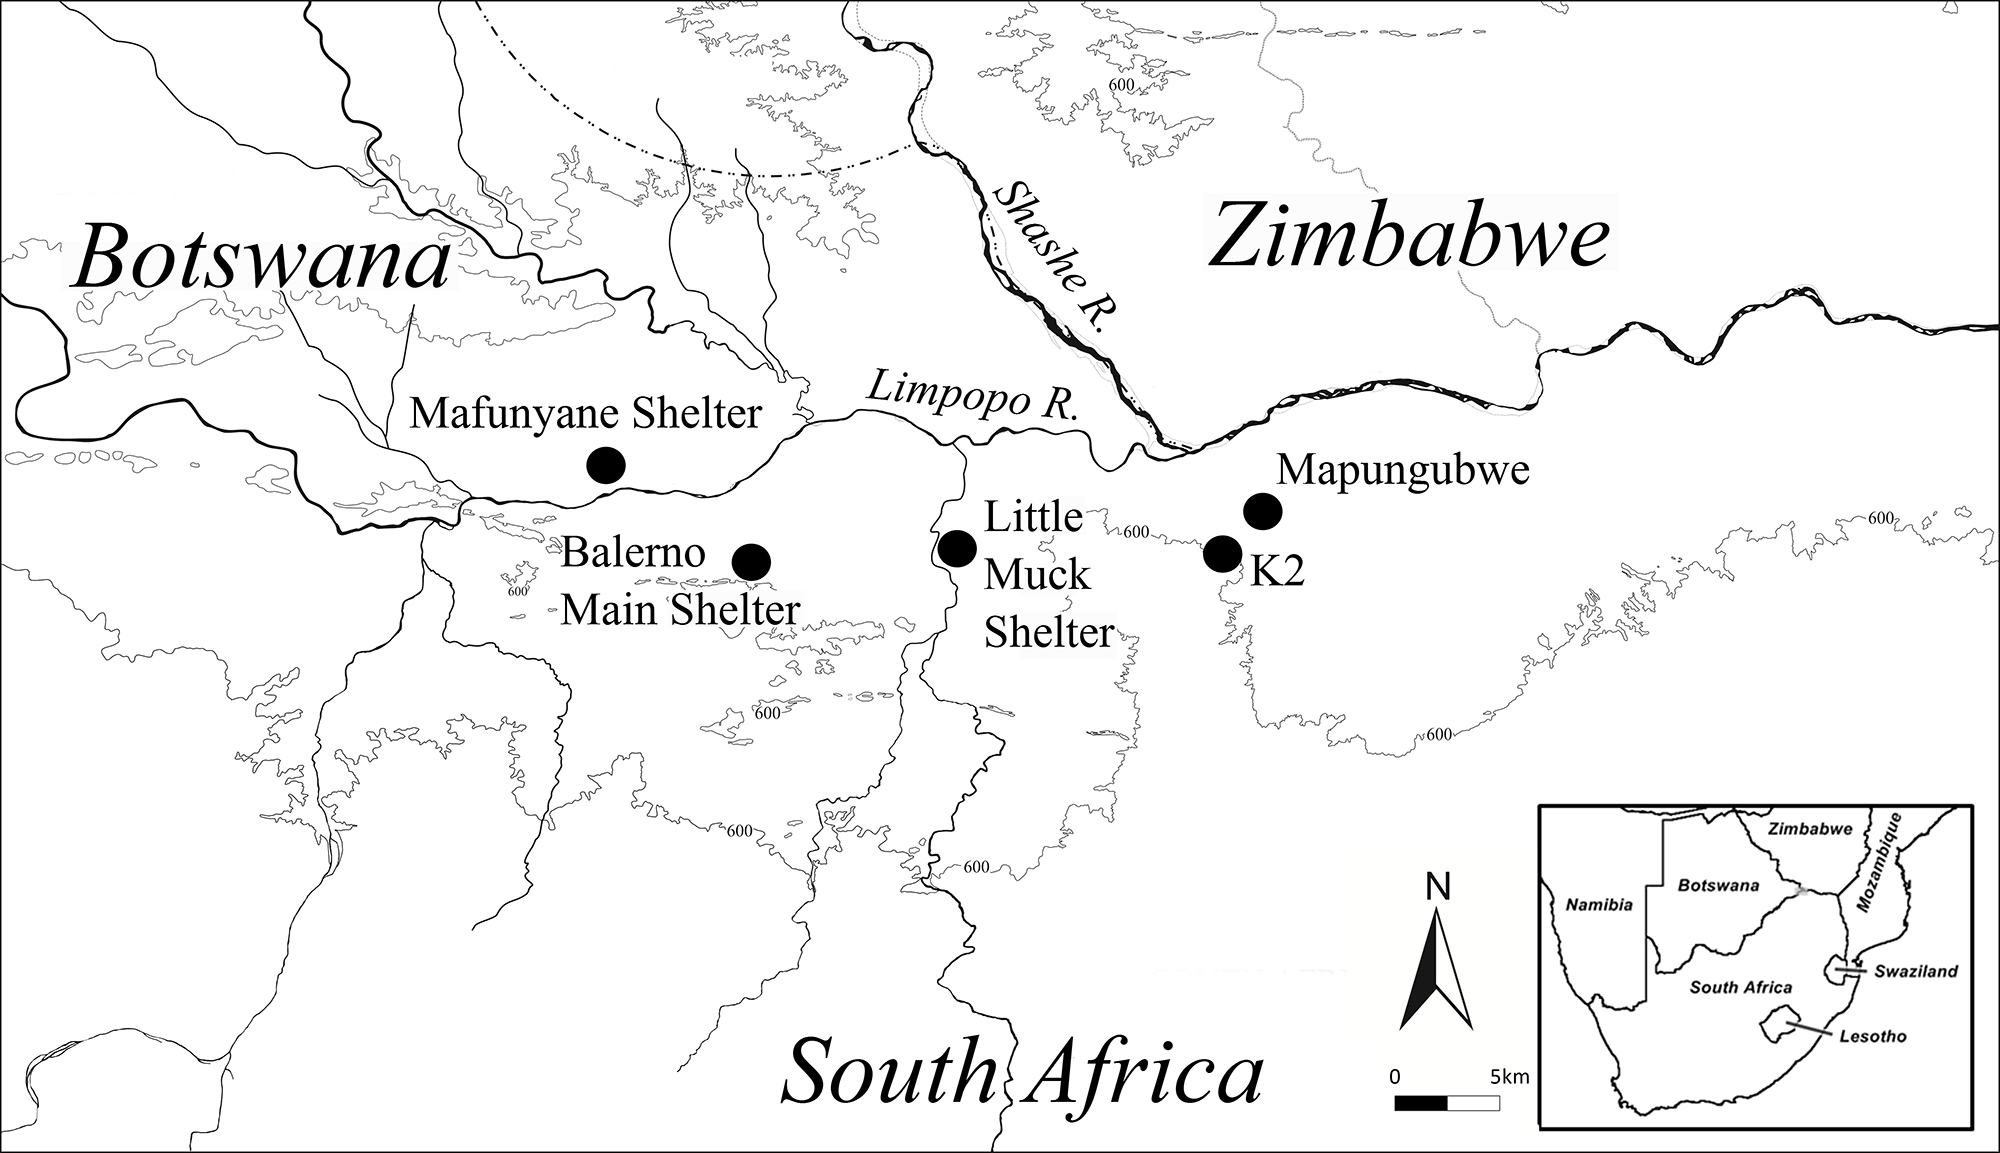
\includegraphics[width=\linewidth]{../figures/Forssman-Figure01}
		\caption{The Greater Mapungubwe Landscape with sites mentioned in the text and other prominent sites.}
		\label{fig:Forssmann-Figure01}
\end{figure}
	
	\section{Mafunyane Shelter}
	
	Mafunyane is situated in a sandstone belt that stretches along the Motloutse, Limpopo, and Shashe Rivers. Within this area are low-lying koppies (sandstone inselbergs) and ridges interspersed with water networks and small floodplains. The area immediately surrounding the site is characterised by a fine loam to clay soil horizon, created by depositional processes from flooding by the Limpopo River, \SI{460}{\meter} away, and a nearby seasonal stream. The vegetation around the site is characterised by dense pockets of mopane veld (\emph{Colophospermum mopane}) and more widespread vachellia and acacia open shrubland. The site’s near proximity to the Limpopo River suggests that in the past the immediate area may have been a riverine woodland, which today is restricted to the banks of major rivers due to the receding water table \parencite{Alexander_1984}.
	
	\textcite{Walker_1994} previously excavated the site under the name Tuli Lodge. It was not known at first whether Mafunyane was \textcite['s]{Walker_1994} site because no GPS co-ordinates were published and at the time of this study the reserve management had not been informed of his research on the farm. Once it was established that the sites were the same it was decided to re-excavate the rockshelter in order to increase the site’s sample size, obtain charcoal samples for radiocarbon dating and relate the findings made here to the broader regional sequence. \textcite['s]{Walker_1994} study revealed an extensive LSA assemblage including \num{14,379} stone tools along with 21 pieces of worked bone, fragments from tortoise and ostrich eggshell bowls and containers, 67 ostrich eggshell beads, 64 potsherds, a pipe and crucible, six glass trade beads and 16 metal implements as well as large amounts of metal prills. He concluded that based on the prevalence of scrapers in the assemblage, the site was occupied quite late, probably from the first few centuries\AD, and that the foragers using the site were in contact with farmers. In addition, he states that the rockshelter was ‘clearly a major living site’ that ‘was probably seasonally occupied, but it was later used by metalworking people to smelt copper’ \textcite[10]{Walker_1994}. 
	
\section{Excavation, Stratigraphy, and Chronology}

The site’s floor was divided into a grid of \SIrange{1}{1}{\meter} squares with alphabetical designations running east to west and numeric designations running south to north. 
Square 3C was selected for excavations primarily because it was located in an area most likely to contain a deep and intact deposit (Fig. \ref{fig:Forssman-Figure02}). 
On excavating the square it was found that a portion of it, the southwestern quadrant, protruded into what appeared to be \textcite['s]{Walker_1994} excavation and so this quadrant was excluded; thus only three quadrants were excavated to bedrock. Initially excavations were also to be conducted in the large open-air living area north of the site, but this area was found to contain little deposit and appeared highly disturbed. 
Excavations therefore only proceeded inside the rockshelter and were conducted in spits of \SI{30}{\milli\meter} following natural stratigraphic units.

	\begin{figure}
		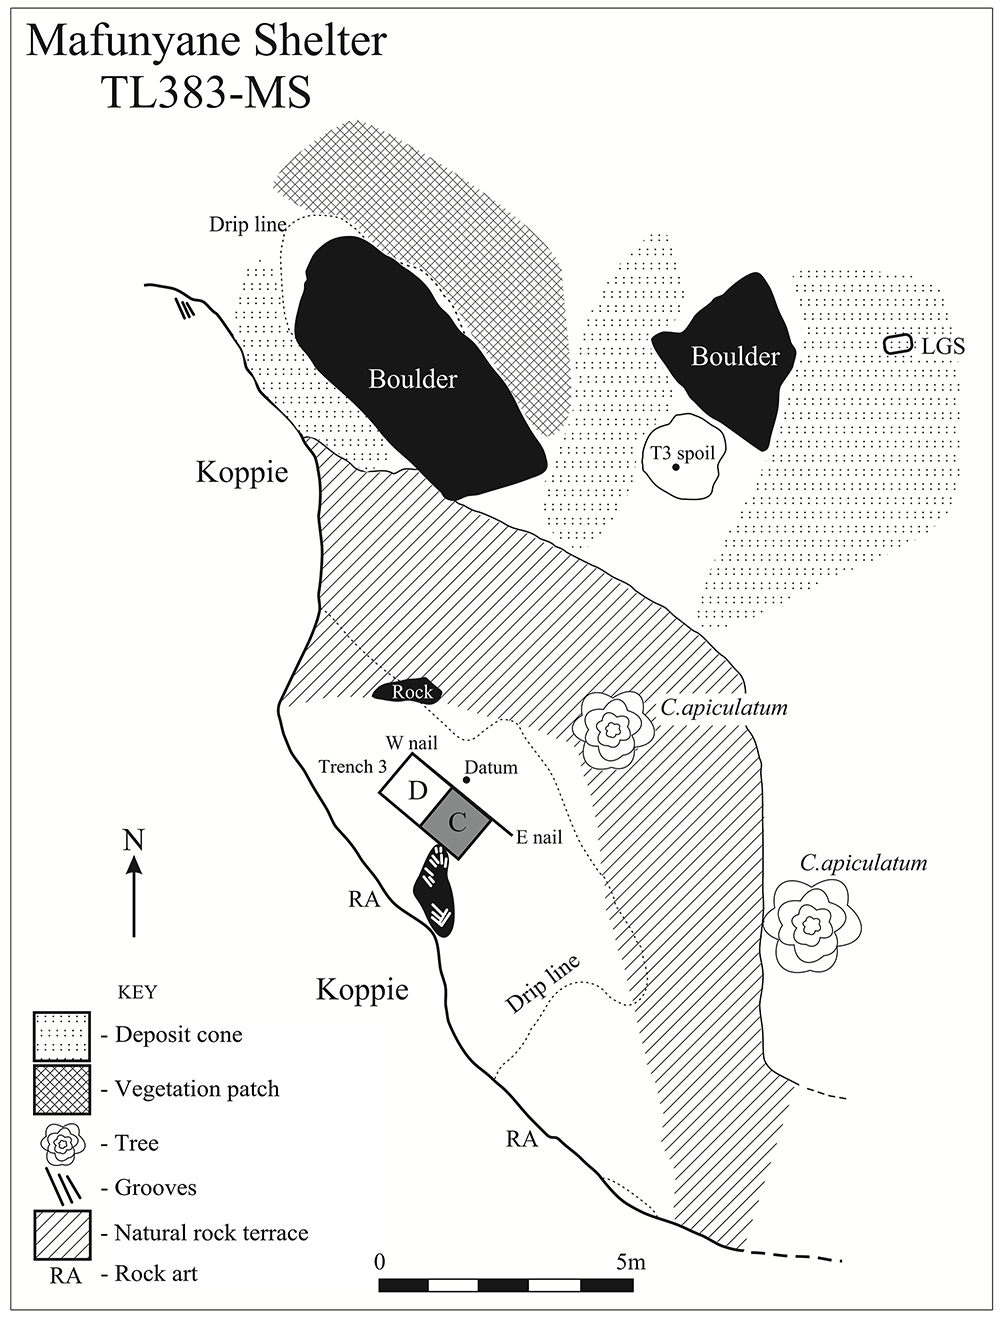
\includegraphics[width=\linewidth]{../figures/Forssman-Figure02.png}
		\caption{Only Square C was excavated at Mafunyane since Square D protruded into \textcite['s]{Walker_1994} excavation, not visible on the surface but recorded once the surface layer was removed \parencite[from][96]{Forssman_2014a}.}
		\label{fig:Forssmann-Figure02}
	\end{figure}

In total seven spits between the surface and bedrock were excavated, revealing three stratigraphic layers, each distinct from the other and similar to \textcite['s]{Walker_1994}. 
The upper most layer, Pale brown sand (PBS), contains small (<\SI{25}{\milli\meter}) sandstone pebbles in an unconsolidated deposit, less than 6 cm thick filling 2.3 buckets (\SI{13}{\liter} each). 
PBS occurred in Spit I-III but from Spit II, Ashy sand (AS) appears and may be a hearth layer. This layer is ash grey, loosely consolidated, with few to no pebbles and is also about \SI{6}{\centi\meter} in thickness (3.4 buckets). 
The lowermost layer, Stony-ashy sand (SAS), is the most substantial (± \SI{12}{\centi\meter} in thickness; 4.5 buckets) and also appears to be a hearth with a similar colour to AS but with considerably more pebbles and stones included in the deposit (Fig. \ref{fig:Figure 03}); the depth of bedrock was on average \SI{20}{\centi\meter} below the surface and a total of 10.3 buckets was removed from the site \parencite[for more details see][95]{Forssman 2014a}. 

Two charcoal samples were submitted for radiocarbon dating to Beta Analytic and the results are presented in Fig. \ref{fig:Forssmann-Table 01}. The samples indicate that the site was occupied between \AD 941 and 1265. However, the more recent date is from Spit VII and the older from Spit II. The laboratory did not find any evidence indicating that the samples were possibly contaminated and so this does not seem to have caused the inverted dates. It is possible that the sample from Spit VII is ‘old wood’, which introduces an unresolvable variable into the calibration process \parencite{Kennett_2002}, but could equally have moved after deposition, possibly due to bioturbation \parencite[see][]{Lancaster_2003} or root action in the deposit (roots were recorded above bedrock). Ceramics do little to assist, although they appear to be contemporaneous (discussed below), and no other chronological markers were identified in the relevant spits. Therefore, the integrity of the deposit is uncertain (but see discussion below).

	\begin{figure} %FIGURE 4 or TABLE 1
		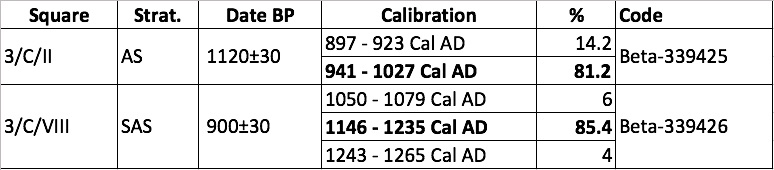
\includegraphics[width=\linewidth]{../figures/Forssman-Table01.png}
		\captionof{table}{Calibrated radiocarbon dates on charcoal samples from Mafunyane.}
		\label{fig:Forssmann-Table01}
	\end{figure}

\section{The Stone Tool Assemblage}

Square C produced a total of \num{6349} stone tools within 10.3 buckets (\SI{0.1}{\meter\cubed}). 
As with other rockshelter excavations in the area, the assemblage is dominated by crypto-crystalline silicates (CCS), after which quartz follows and then consistently low frequencies of quartzite, agate and dolerite. The greatest number of stone artefacts is found between Spits II and V (Fig. \ref{fig:Figure 04}), 
followed by a decrease until bedrock is reached in Spit VII (Fig. \ref{fig:Forssman-Table02}). 
A similar pattern was noted with regard to the stone tool density (artefacts/13l bucket) with the exception of the high density on the surface and in Spit I. If the high density of stone tools on the surface represents a forager use of the rockshelter, it may be after \AD 1200 based on the radiocarbon dates and the Leopard’s Kopje ceramics found by \textcite{Walker_1994} in the upper levels of his excavation. 

	\begin{figure} %Figure 5
		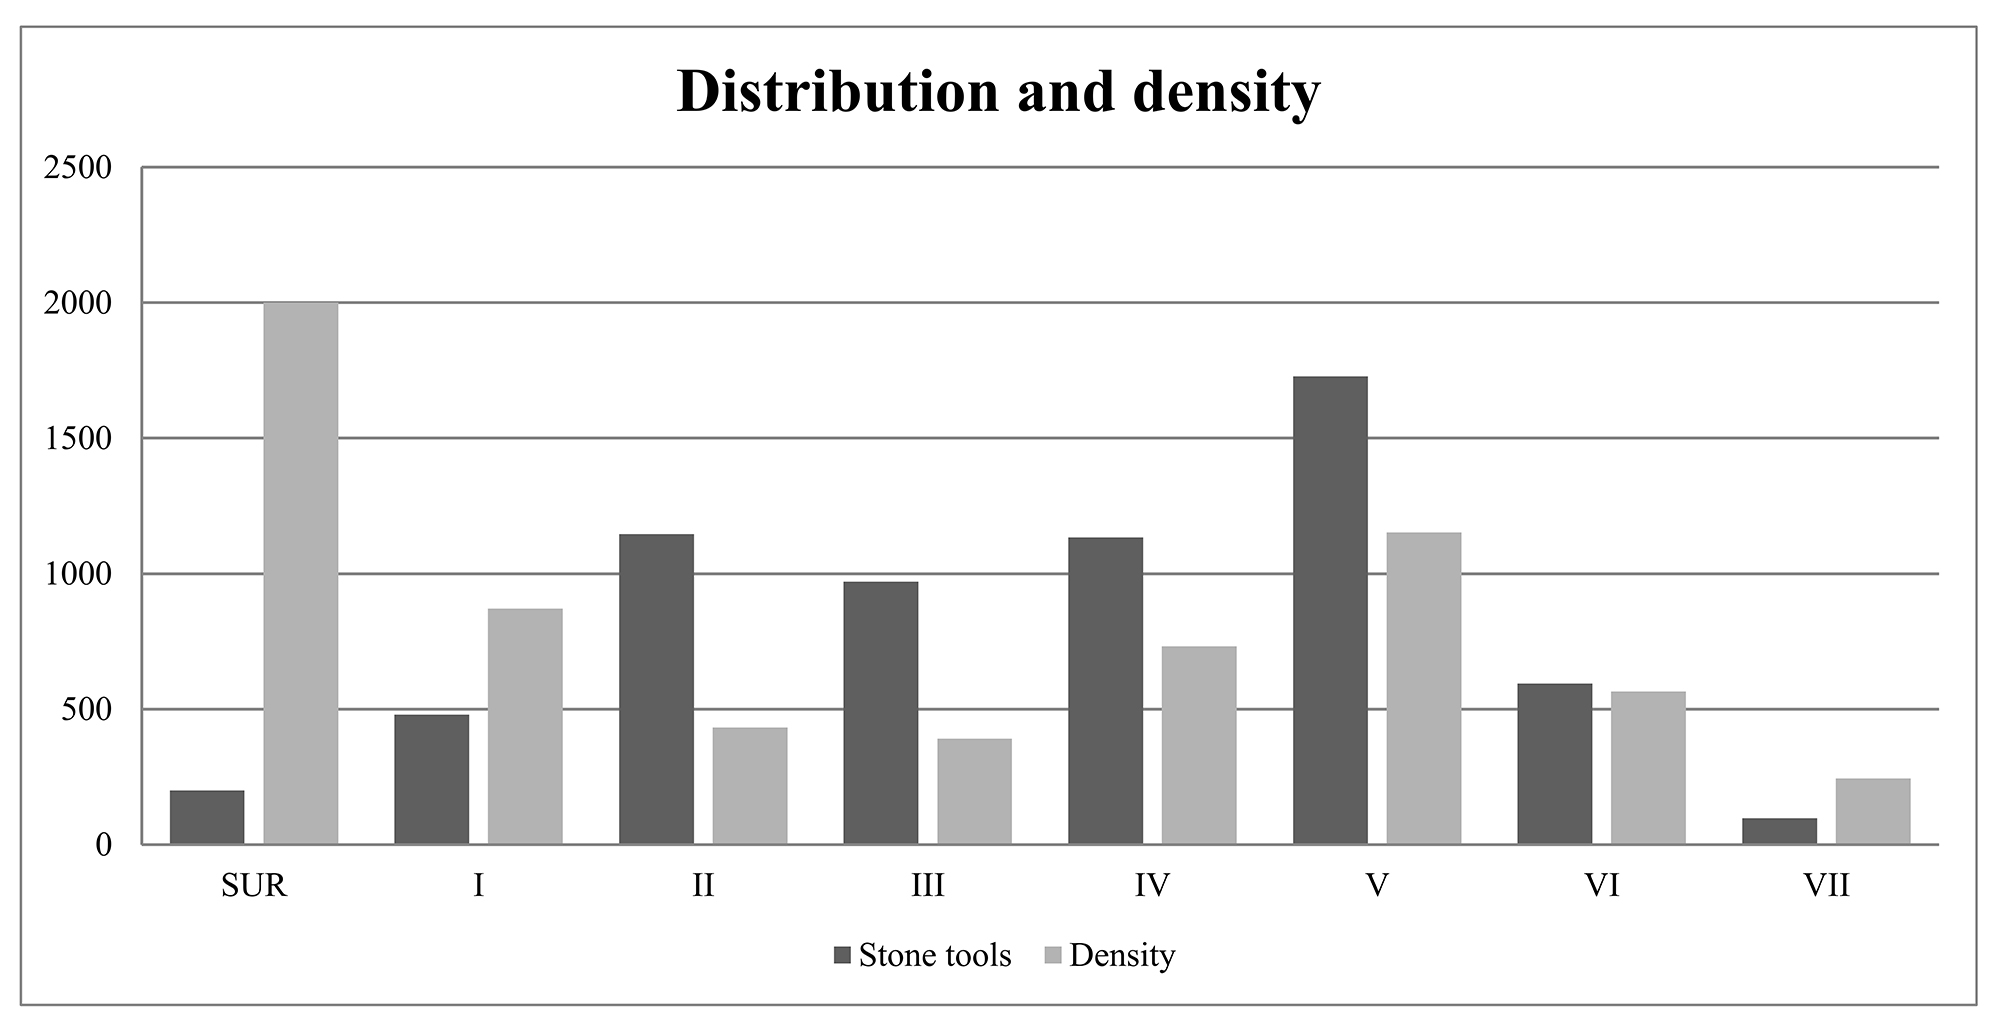
\includegraphics[width=\linewidth]{../figures/Forssman-Figure04.png}
		\caption{Only Square C was excavated at Mafunyane since Square D protruded into \textcite['s]{Walker_1994} excavation, not visible on the surface but recorded once the surface layer was removed \parencite[from][96]{Forssman_2014a}.}
		\label{fig:Forsmann-Figure04}
	\end{figure}

Below the stone tool assemblage has been separated into two categories based on \textcite['s]{Walker_1994} typological breakdown: 1) debitage and utilised pieces and 2) formal tools.

	\begin{figure} %FIGURE 6 or TABLE 2
		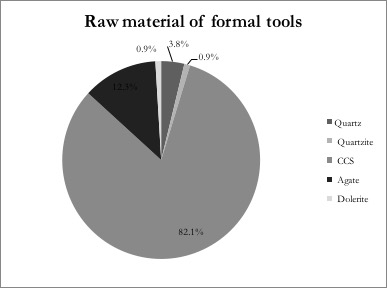
\includegraphics[width=\linewidth]{../figures/Forssman-Table02.png}
		\captionof{table}{Calibrated radiocarbon dates on charcoal samples from Mafunyane.}
		\label{fig:Forssman-Table02}
	\end{figure}

	%----------------------------------------------------------------------------------------
	
	\printbibliography[heading=subbibnumbered] 
	\label{Forssman:lastpage}
%------------------------------------------------------------------------------
\closingarticle